% ============================================================
% 西安交通大学博士/硕士学位论文模板（完整合并版，含页码注释）
% 编译方式：XeLaTeX
% ============================================================

\documentclass[UTF8, scheme=chinese, openany, oneside]{ctexbook}

% ------------------------------------------------------------
% 必要宏包
% ------------------------------------------------------------
\usepackage{geometry}
\geometry{top=3.5cm, bottom=2.5cm, left=3cm, right=2.5cm, headheight=1.5cm}
\usepackage{xcolor}
\usepackage[most]{tcolorbox}
\usepackage{setspace}
\usepackage{fancyhdr}
\usepackage{titletoc}
\usepackage{graphicx}
\usepackage{amsmath, amssymb}
\usepackage{booktabs}
\usepackage{tabularx}
\usepackage{multirow}
\usepackage{enumitem}
\usepackage[super, square, sort&compress]{natbib}
\usepackage{bicaption}
\usepackage{pifont} % 提供圈码脚注

% ------------------------------------------------------------
% 字体设置（使用项目自带字体）
% ------------------------------------------------------------
\setmainfont{NimbusRoman-Regular.otf}[
    Path=font/,
    BoldFont=NimbusRoman-Bold.otf,
    ItalicFont=NimbusRoman-Italic.otf,
    BoldItalicFont=NimbusRoman-BoldItalic.otf
]
\setCJKmainfont{NotoSerifCJK-Regular.ttc}[
    Path=font/,
    BoldFont=NotoSerifCJK-Bold.ttc
]
\setCJKsansfont{NotoSansCJK-Regular.ttc}[
    Path=font/,
    BoldFont=NotoSansCJK-Bold.ttc
]
\newcommand{\sanhao}{\zihao{3}}
\newcommand{\sihao}{\zihao{4}}
\newcommand{\xiaosi}{\zihao{-4}}
\newcommand{\wuhao}{\zihao{5}}
\newcommand{\xiaowu}{\zihao{-5}}

% ------------------------------------------------------------
% 论文基本信息
% ------------------------------------------------------------
\title{XXXXXXXXXXXXXXXXXXXX（论文题目不能超过35个汉字）}
\author{XXX}
\newcommand{\university}[1]{\def\@university{#1}}
\newcommand{\college}[1]{\def\@college{#1}}
\newcommand{\major}[1]{\def\@major{#1}}
\newcommand{\advisor}[1]{\def\@advisor{#1}}
\newcommand{\studentid}[1]{\def\@studentid{#1}}
\newcommand{\degree}[1]{\def\@degree{#1}}
\newcommand{\submitdate}[1]{\def\@submitdate{#1}}
\newcommand{\englishtitle}[1]{\def\@englishtitle{#1}}
\newcommand{\englishauthor}[1]{\def\@englishauthor{#1}}
\newcommand{\englishadvisor}[1]{\def\@englishadvisor{#1}}
\newcommand{\thesistype}[1]{\def\@thesistype{#1}}
\university{西安交通大学}
\college{XX学院}
\major{XX专业}
\advisor{XXX教授}
\studentid{20XXXXXXXX}
\degree{硕士学位论文}
\submitdate{XXXX年XX月}
\englishtitle{XXXXXXXXXXXXXXXXXXXXXXXXXXXXXXXXXXXXXXXXXXXXXX}
\englishauthor{XXX}
\englishadvisor{Prof. XXX}
\thesistype{应用研究}

\makeatletter
\newif\if@doctor
\@doctorfalse % 硕士
\makeatother

% ------------------------------------------------------------
% 封面、英文标题页、答辩委员会页命令
% ------------------------------------------------------------
\newcommand{\makecover}{%
    \begin{titlepage}
        \centering
        \vspace*{2cm}
        {\sanhao\sffamily\bfseries \@university}\\
        \vspace{1cm}
        {\sanhao\sffamily\bfseries \@degree}\\
        \vspace{3cm}
        {\sihao\bfseries \@title}\\
        \vspace{3cm}
        {\xiaosi
        \begin{tabular}{l}
            学科专业：\@major\\
            作者姓名：\@author\\
            指导教师：\@advisor\\
            学\qquad 号：\@studentid\\
            提交日期：\@submitdate
        \end{tabular}}
        \vfill
    \end{titlepage}
}

\newcommand{\makeenglishtitle}{%
    \begin{titlepage}
        \centering
        \vspace*{2cm}
        {\sanhao\bfseries \@englishtitle}\\
        \vspace{3cm}
        {\xiaosi
        \begin{tabular}{l}
            Discipline: \@major\\
            Candidate: \@englishauthor\\
            Supervisor: \@englishadvisor\\
            Date: \@submitdate
        \end{tabular}}
        \vfill
    \end{titlepage}
}

\newcommand{\makedefensecommittee}{%
    \clearpage
    \chapter*{博士/硕士学位论文答辩委员会}
    \addcontentsline{toc}{chapter}{答辩委员会}
    \begin{center}
        {\sihao\bfseries \@title}
    \end{center}
    \vspace{0.5cm}
    \noindent 答辩人：\@author\\
    \vspace{0.3cm}
    \noindent 答辩委员会委员：\\
    \begin{tabular}{lll}
        XXXXXXXXXX大学XXX: & （主席）\\
        XXXXXXXXXX大学XXX: & \\
        XXXXXXXXXX大学XXX: & \\
        XXXXXXXXXX大学XXX: & \\
        XXXXXXXXXX大学XXX: & 
    \end{tabular}\\
    \vspace{0.5cm}
    \noindent 答辩时间：XXXX年XX月XX日\\
    答辩地点：XXXXXX
}

% ------------------------------------------------------------
% 页眉样式
% ------------------------------------------------------------

% 双横线页眉样式（用于摘要页）
\fancypagestyle{doublelinestyle}{
    \fancyhf{}
    \fancyhead[C]{\zihao{5}摘\quad 要}
    \fancyfoot[C]{}
    \renewcommand{\headrulewidth}{0.4pt}
    \renewcommand{\headrule}{%
        \hrule width\headwidth height\headrulewidth\vskip 2pt%
        \hrule width\headwidth height\headrulewidth%
    }
}

% 双横线页眉样式（用于致谢页）
\fancypagestyle{ackdoublelinestyle}{
    \fancyhf{}
    \fancyhead[C]{\zihao{5}致\quad 谢}
    \fancyfoot[C]{}
    \renewcommand{\headrulewidth}{0.4pt}
    \renewcommand{\headrule}{%
        \hrule width\headwidth height\headrulewidth\vskip 2pt%
        \hrule width\headwidth height\headrulewidth%
    }
}

% 双横线页眉样式（用于参考文献第一页和奇数页）
\fancypagestyle{refdoublelinestyle}{
    \fancyhf{}
    \fancyhead[C]{\zihao{5}参考文献}
    \fancyfoot[C]{}
    \renewcommand{\headrulewidth}{0.4pt}
    \renewcommand{\headrule}{%
        \hrule width\headwidth height\headrulewidth\vskip 2pt%
        \hrule width\headwidth height\headrulewidth%
    }
}

\fancypagestyle{frontmatterstyle}{
    \fancyhf{}
    \fancyhead[CO]{\zihao{5}摘要}
    \fancyhead[CE]{\zihao{5}\@university\if@doctor 博士\else 硕士\fi 学位论文}
    \fancyfoot[C]{\thepage}
    \renewcommand{\headrulewidth}{0.4pt}
}
\fancypagestyle{mainmatterstyle}{
    \fancyhf{}
    \fancyhead[CO]{\zihao{5}\leftmark}
    \fancyhead[CE]{\zihao{5}\@university\if@doctor 博士\else 硕士\fi 学位论文}
    \fancyfoot[C]{\thepage}
    \renewcommand{\headrulewidth}{0.4pt}
}
\fancypagestyle{backmatterstyle}{
    \fancyhf{}
    \fancyhead[CO]{\zihao{5}\leftmark}
    \fancyhead[CE]{\zihao{5}\@university\if@doctor 博士\else 硕士\fi 学位论文}
    \fancyfoot[C]{\thepage}
    \renewcommand{\headrulewidth}{0.4pt}
}

% 蓝色说明框
\newtcolorbox{noticebox}{
    colback=white,
    colframe=blue,
    boxrule=1.5pt,
    sharp corners,
    halign=flush left,
    before skip=1cm,
    after skip=1cm,
    title=\colorbox{red}{\color{white}{\bfseries \zihao{5} 说明}},
    colbacktitle=white,
    attach boxed title to top center={yshift=-2mm},
    boxed title style={empty, boxrule=0pt}
}

% ------------------------------------------------------------
% 用户添加的绪论章节样式设置
% ------------------------------------------------------------

% --- 页面样式设置 ---
\fancypagestyle{pageone}{
    \fancyhf{}
    \fancyhead[C]{\zihao{5} 1 \quad 绪论}
    \fancyfoot[R]{\zihao{-5} \thepage}
    \renewcommand{\headrulewidth}{0.6pt}
}

\fancypagestyle{pagetwo}{
    \fancyhf{}
    \fancyhead[C]{\zihao{5} 西安交通大学博士/硕士学位论文}
    \fancyfoot[L]{\zihao{-5} \thepage}
    \renewcommand{\headrulewidth}{0.6pt}
}

% --- 脚注样式修改：1/4线宽，圈码 ---
\renewcommand{\thefootnote}{\ding{\numexpr171+\value{footnote}}}
\renewcommand{\footnoterule}{
    \noindent\rule{0.25\textwidth}{0.4pt}\vspace{2pt}
}

% --- 段落与间距 ---
\setstretch{1.5} % 行间距 1.5
\ctexset{
    section = {
        format = \zihao{4}\bfseries\raggedright,
        number = \arabic{chapter}.\arabic{section},
        indent = 0em,
    },
    subsection = {
        format = \zihao{-4}\bfseries\raggedright,
        number = \arabic{chapter}.\arabic{subsection},
        indent = 0.5em,
    },
    subsubsection = {
        format = \zihao{-4}\bfseries\raggedright,
        number = \arabic{chapter}.\arabic{subsection}.\arabic{subsubsection},
        indent = 0.5em,
    }
}

% --- 列表样式自定义（4-7级标题缩进控制）---
% 第4级：1) 标题 4 —— 缩进 0.5em
\newlist{levelfour}{enumerate}{1}
\setlist[levelfour]{
    label=\arabic*),
    align=left,
    labelindent=0.5em,
    leftmargin=*,
    itemsep=0pt,
    parsep=0pt,
    topsep=0.5em
}

% 第5级：(1) 标题 5 —— 缩进 1em
\newlist{levelfive}{enumerate}{1}
\setlist[levelfive]{
    label=(\arabic*),
    align=left,
    labelindent=1em,
    leftmargin=*,
    itemsep=0pt,
    parsep=0pt,
    topsep=0.5em
}

% 第6级：a) 标题 6 —— 缩进 2em
\newlist{levelsix}{enumerate}{1}
\setlist[levelsix]{
    label=\alph*),
    align=left,
    labelindent=2em,
    leftmargin=*,
    itemsep=0pt,
    parsep=0pt,
    topsep=0.5em
}

% 第7级：(a) 标题 7 —— 缩进 2.5em
\newlist{levelseven}{enumerate}{1}
\setlist[levelseven]{
    label=(\alph*),
    align=left,
    labelindent=2.5em,
    leftmargin=*,
    itemsep=0pt,
    parsep=0pt,
    topsep=0.5em
}

% ============================================================
% 正文开始
% ============================================================
\begin{document}
\renewcommand*{\citenumfont}[1]{[#1]}

% ============================================================
% 新增第1页：中文题名页（预留页）- 对应PDF第1页
% ============================================================
\clearpage
\thispagestyle{empty}
\vspace*{5.8cm}  % 页面顶端到蓝色框最上面距离
\begin{center}
\begin{tcolorbox}[
    colback=white,
    colframe=blue,
    boxrule=1.5pt,
    sharp corners,
    width=0.8\textwidth,
    center,
    halign=center
]
    {\sffamily\bfseries\zihao{3}\textcolor{red}{中文题名页 预留页}}\\[0.5cm]
    {\rmfamily\zihao{5}拆入内容前删除此框}
\end{tcolorbox}
\end{center}
\vfill

% ============================================================
% 新增第2页：英文题名页（预留页）- 对应PDF第3页
% ============================================================
\clearpage
\thispagestyle{empty}
\vspace*{5.8cm}
\begin{center}
\begin{tcolorbox}[
    colback=white,
    colframe=blue,
    boxrule=1.5pt,
    sharp corners,
    width=0.8\textwidth,
    center,
    halign=center
]
    {\sffamily\bfseries\zihao{3}\textcolor{red}{英文题名页 预留页}}\\[0.5cm]
    {\rmfamily\zihao{5}拆入内容前删除此框}
\end{tcolorbox}
\end{center}
\vfill

% ============================================================
% 第3页：博士/硕士学位论文答辩委员会
% ============================================================
\clearpage
\thispagestyle{empty}

\begin{center}
\begin{tcolorbox}[
    colback=white, colframe=blue, boxrule=1.5pt, sharp corners,
    width=0.8\textwidth, center, halign=center,
    top=2mm, bottom=2mm
]
    {\rmfamily\zihao{5}请根据学位层级选择下面的博士或硕士，阅后删除此框}
\end{tcolorbox}
\end{center}

\vspace{0.5cm} 

\begin{center}
    {\rmfamily\bfseries\zihao{4} 博士/硕士学位论文答辩委员会}
\end{center}

% 2. 标题与论文题目之间距离约 1cm
\vspace{1cm} 

\begin{center}
    {\fontsize{15.9pt}{19pt}\selectfont\bfseries XXXXXXXXXXXXXXXXXXXX（论文题目不能超过 35 个汉字）}
\end{center}

% 3. 论文题目到答辩人之间距离约 4cm
\vspace{4cm} 

% 答辩人：距离左边界约 2.5cm
\noindent\hspace{2.5cm}{\rmfamily\zihao{5} 答辩人：XXX}\\[0.4cm]

% 答辩委员会委员：与答辩人对齐
\noindent\hspace{2.5cm}{\rmfamily\zihao{5} 答辩委员会委员：}\\[0.4cm]

% 4. 委员名单：使用 tabular 精确对齐
% 整体再缩进约 1.5cm，使委员名单比"答辩委员会委员"更靠右
\noindent\hspace{4cm}%
\begin{tabular}{@{}l@{}l@{}l@{}}
    {\rmfamily\zihao{5} XXXXXXXXXX 大学 XXX：} & {\rmfamily\zihao{5} \underline{\hspace{3.5cm}}} & {\color{red}\rmfamily\zihao{5}（注：主席）} \\[0.25cm]
    {\rmfamily\zihao{5} XXXXXXXXXX 大学 XXX：} & {\rmfamily\zihao{5} \underline{\hspace{3.5cm}}} & \\[0.25cm]
    {\rmfamily\zihao{5} XXXXXXXXXX 大学 XXX：} & {\rmfamily\zihao{5} \underline{\hspace{3.5cm}}} & \\[0.25cm]
    {\rmfamily\zihao{5} XXXXXXXXXX 大学 XXX：} & {\rmfamily\zihao{5} \underline{\hspace{3.5cm}}} & \\[0.25cm]
    {\rmfamily\zihao{5} XXXXXXXXXX 大学 XXX：} & {\rmfamily\zihao{5} \underline{\hspace{3.5cm}}} & \\
\end{tabular}

\vfill

\clearpage
\thispagestyle{empty}

\vfill  % 保持垂直居中

% 答辩时间和地点格式与第三页答辩人、答辩委员会委员保持一致
\noindent\hspace{2.5cm}{\rmfamily\zihao{5} 答辩时间：XXXX 年 XX 月 XX 日}\\[0.4cm]

\noindent\hspace{2.5cm}{\rmfamily\zihao{5} 答辩地点：XXXXXX}

\vfill


% ------------------------------------------------------------
% 第I页：中文摘要
% ------------------------------------------------------------
\clearpage
\frontmatter
\thispagestyle{doublelinestyle} % 假设这是您定义好的带有页眉横线的样式
\pagestyle{doublelinestyle}

% 1. 中文摘要标题 (三号，黑体/微软雅黑，居中，不加粗)
\begin{center}
    \vspace*{0.05cm} % 紧贴页眉线
    {\zihao{3}\sffamily 摘\quad 要}
\end{center}
\addcontentsline{toc}{chapter}{摘要}
\vspace{0.6cm} % 标题下方间距

% 2. 摘要说明文字 (行间距建议设置，保持段落感)
{\zihao{-4}\kaishu % 模板通常使用楷体或宋体说明，这里根据图片视觉微调
论文摘要由摘要正文、关键词、论文类型、资助申明等部分组成。

博士学位论文摘要正文为 1000 字(word)左右，硕士学位论文摘要正文为 600 字(word)左右。

内容一般包括：从事这项研究工作的目的和意义；完成的工作（作者独立进行的
研究工作及相应结果的概括性叙述）；获得的主要结论（这是摘要的中心内容）。博
士学位论文摘要应突出论文的创新点，硕士学位论文摘要应突出论文的新见解。

摘要中一般不用图、表、化学结构式、非公知公用的符号和术语。

如果论文的主体工作得到了有关基金资助，应在摘要第一页的页脚处标注：本研
究得到某某基金（编号：）资助。（五号）
}

% 3. 省略号部分 (精确间距控制)
\vspace{1.58cm}
\begin{center}
    $\dots\dots$
\end{center}
\vspace{1.58cm}

% 4. 关键词部分
\noindent{\color{red}\bfseries 关\ 键\ 词：}{\rmfamily XXX；XXX；XXX\textsuperscript{*}；XXX；XXX}

\vspace{0.3cm}

% 关键词说明文字（缩进两个字符）
{\zihao{5}
\noindent\hspace{2em}关键词由3～5个组成。关键词应从《汉语主题词表》中摘选，当《汉语主题词表》的词不足以反映主题时，可由申请人设计关键词，但须加注。每一关键词之间用分号分开，最后一个关键词后不打标点符号。由申请人设计的关键词，须在该关键词的右上角标注*，并在该页的页脚处注明“*表示非汉语主题词”。
}

\vspace{0.8cm}

% 5. 论文类型部分
\noindent{\color{red}\bfseries 论文类型：}{\rmfamily XXXX}

\vspace{0.3cm}
{\zihao{5} \noindent 论文类型包括：a.理论研究（Theoretical Research)；b.应用基础(Application Fundamentals)；c. 应用研究(Application Research)；d.研究报告(Research Report)；e.设计报告(Design Report)；f.案例分
析(Case Study)；g.调研报告(Investigation Report)；h.产品研发(Product Development)；i.工程设计
(Engineering Design)；j.工程/项目管理(Engineering/Project Management)；k.其它（Others）。}



% ------------------------------------------------------------
% ------------------------------------------------------------
% 第II页：英文摘要 (ABSTRACT)
% ------------------------------------------------------------
\clearpage
\pagenumbering{Roman} % 确保页码为罗马数字
\setcounter{page}{2}  % 设为第二页 II

% --- 页眉设置 ---
\pagestyle{fancy}
\fancyhf{}
\fancyhead[C]{\zihao{5} ABSTRACT} % 页眉改为 ABSTRACT
\renewcommand{\headrulewidth}{0.75pt} % 页眉横线

% --- 1. 蓝色提示框 ---
\begin{center}
    \begin{tcolorbox}[
        colback=white, 
        colframe=blue, 
        boxrule=1.5pt, 
        sharp corners, 
        width=0.85\textwidth,
        center,
        halign=center,
        top=2mm, bottom=2mm
    ]
        {\rmfamily\zihao{4} 请注意选择页眉中相应的学位层次，阅后{\color{red}删除此框}}
    \end{tcolorbox}
\end{center}

% --- 2. 标题 ---
\vspace{0.5cm}
\begin{center}
    {\zihao{3} ABSTRACT}
\end{center}
\addcontentsline{toc}{chapter}{ABSTRACT}
\vspace{0.5cm}

% --- 3. 指导性文字 (严格还原图片内容) ---
\noindent {\zihao{-4} 英文摘要撰写要求如下：}

\noindent {\zihao{-4} （1）用词准确，符合语法；}

\noindent {\zihao{-4} （2）关键词按相应专业的标准术语写出，尽量从《英语主题词表》中摘选；}

\noindent {\zihao{-4} （3）如果论文的主体工作得到了有关基金资助，应用英文在摘要第一页的页脚处标注：本研究得到某某基金（编号：）资助；}

\vspace{0.3cm}
\noindent {\zihao{-4} 中文摘要和英文摘要均不要求学位申请人及其指导教师签字。}

\vspace{0.3cm}
\noindent {\zihao{-4} 摘要正文每段{\color{red}开头不空格}，{\color{red}每段之间空一行}；}

\vspace{1cm}

% --- 4. 摘要正文 (严格还原占位文字，设置不缩进且段间距) ---
\setlength{\parindent}{0pt}          % 全局设置本页不缩进
\setlength{\parskip}{1em}             % 设置段间距为1行

{\zihao{-4}
The key parts in drip irrigation facilities are emitters. The structural design parameters of emitters can directly affect its performance and the function of the whole drip irrigation system ......

1. Because......

2. Only ......

3. To support ......
}

\vspace{1cm}

% --- 5. KEY WORDS 部分 ---
\noindent {\zihao{-4}\bfseries KEY WORDS: XXX; XXX; XXX; XXX}

\noindent {\zihao{5} 每个关键词组的第一个字母大写，其余为小写，每一关键词之间用分号分开，最后一个关键词后不打标点符号。例如：Drip irrigation emitter; RP\&M; Hydraulics; Labyrinth flow channel}

\vspace{0.8cm}

% --- 6. TYPE OF DISSERTATION 部分 ---
\noindent {\zihao{-4}\bfseries TYPE OF DISSERTATION: XXXXXXX}

\noindent {\zihao{5} 须与中文摘要中的论文类型一致；每个单词第一个字母大写，其余为小写。例如：Applied Research}

\noindent {\zihao{5} 论文类型包括：a.理论研究（Theoretical Research)；b.应用基础(Application Fundamentals)；c.应用研究(Application Research)；d.研究报告(Research Report)；e.设计报告(Design Report)；f.案例分析(Case Study)；g.调研报告(Investigation Report)；h.产品研发(Product Development)；i.工程设计(Engineering Design)；j.工程/项目管理(Engineering/Project Management)；k.其它（Others）。}

% 页脚页码
\fancyfoot[C]{\zihao{5} II}

% ------------------------------------------------------------
% 第III页：中文目录 (第一页)
% ------------------------------------------------------------
\clearpage
\pagenumbering{Roman}
\setcounter{page}{3} % 设定为 III

% --- 第III页页眉页脚 ---
\fancypagestyle{tocpageIII}{
    \fancyhf{}
    \fancyhead[C]{\zihao{5} 西安交通大学博士/硕士学位论文}
    \fancyfoot[C]{\zihao{5} III} % III 居中
    \renewcommand{\headrulewidth}{0.75pt}
}
\thispagestyle{tocpageIII}

% 目录大标题
\begin{center}
    \vspace*{0.2cm}
    {\zihao{3}\sffamily 目\quad 录}
\end{center}
\vspace{0.4cm}

% --- 目录项排列 ---
\begin{spacing}{1.35} % 调整行间距确保美观，防止溢出
\zihao{5}
\noindent 摘 要 \dotfill I \\
\noindent ABSTRACT \dotfill II \\
\noindent 1 绪论 \dotfill 1 \\
\noindent \hspace*{1.5em} 1.1 标题 2 \dotfill 1 \\
\noindent \hspace*{3.0em} 1.1.1 标题 3 \dotfill 1 \\
\noindent 2 XX（标题 1） \dotfill 6 \\
\noindent \hspace*{1.5em} 2.1 标题 2 \dotfill 6 \\
\noindent \hspace*{3.0em} 2.1.1 标题 3 \dotfill 6 \\
\noindent 3 XXX（标题 1） \dotfill 8 \\
\noindent \hspace*{1.5em} 3.1 标题 2 \dotfill 8 \\
\noindent \hspace*{3.0em} 3.1.1 标题 3 \dotfill 8 \\
\noindent 4 XXXX（标题 1） \dotfill 10 \\
\noindent \hspace*{1.5em} 4.1 标题 2 \dotfill 10 \\
\noindent \hspace*{3.0em} 4.1.1 标题 3 \dotfill 10 \\
\noindent 5 XXXXX（标题 1） \dotfill 12 \\
\noindent \hspace*{1.5em} 5.1 标题 2 \dotfill 12 \\
\noindent \hspace*{3.0em} 5.1.1 标题 3 \dotfill 12 \\
\noindent 6 XXXXXX（标题 1） \dotfill 14 \\
\noindent \hspace*{1.5em} 6.1 标题 2 \dotfill 14 \\
\noindent \hspace*{3.0em} 6.1.1 标题 3 \dotfill 14 \\
\noindent 7 XXXXXXX（标题 1） \dotfill 16 \\
\noindent \hspace*{1.5em} 7.1 标题 2 \dotfill 16 \\
\noindent \hspace*{3.0em} 7.1.1 标题 3 \dotfill 16
\end{spacing}

% ------------------------------------------------------------
% 第IV页：中文目录 (第二页)
% ------------------------------------------------------------
\newpage
\fancypagestyle{tocpageIV}{
    \fancyhf{}
    \fancyhead[C]{\zihao{5} 目\quad 录} % 页眉切换为"目 录"
    \fancyfoot[R]{\zihao{5} IV} % IV 居右
    \renewcommand{\headrulewidth}{0.75pt}
}
\pagestyle{tocpageIV}

\begin{spacing}{1.35}
\zihao{5}
\noindent 8 XXXXXXXX（标题 1） \dotfill 17 \\
\noindent \hspace*{1.5em} 8.1 标题 2 \dotfill 17 \\
\noindent \hspace*{3.0em} 8.1.1 标题 3 \dotfill 17 \\
\noindent 9 XXXXXXXXX（标题 1） \dotfill 19 \\
\noindent \hspace*{1.5em} 9.1 标题 2 \dotfill 19 \\
\noindent \hspace*{3.0em} 9.1.1 标题 3 \dotfill 19 \\
\noindent 10 XXXXXXXXXX（标题 1） \dotfill 21 \\
\noindent \hspace*{1.5em} 10.1 标题 2 \dotfill 21 \\
\noindent \hspace*{3.0em} 10.1.1 标题 3 \dotfill 21 \\
\noindent 11 XXXXXXXXXXX（标题 1） \dotfill 23 \\
\noindent \hspace*{1.5em} 11.1 标题 2 \dotfill 23 \\
\noindent \hspace*{3.0em} 11.1.1 标题 3 \dotfill 23 \\
\noindent 12 结论与展望 \dotfill 25 \\
\noindent \hspace*{1.5em} 12.1 标题 2 \dotfill 25 \\
\noindent \hspace*{3.0em} 12.1.1 标题 3 \dotfill 25 \\
\noindent 致谢 \dotfill 17 \\
\noindent 参考文献 \dotfill 18 \\
\noindent 附录 \dotfill 21 \\
\noindent 攻读学位期间取得的研究成果 \dotfill \\
\noindent 答辩委员会会议决议 \dotfill \\
\noindent 常规评阅人名单 \dotfill \\
\noindent 声明 
\end{spacing}
% ------------------------------------------------------------
% ------------------------------------------------------------
% 第V页：CONTENTS (English Table of Contents)
% ------------------------------------------------------------
\clearpage
\pagenumbering{Roman}
\setcounter{page}{5} % 明确设为第五页

% --- 第V页页眉页脚设置 ---
\pagestyle{fancy}
\fancyhf{}
\fancyhead[C]{\zihao{5} 西安交通大学博士/硕士学位论文}
\fancyfoot[C]{\zihao{5} V} % 第V页码居中
\renewcommand{\headrulewidth}{0.75pt}

% 英文目录大标题（三号，不加粗，居中）
\begin{center}
    \vspace*{0.2cm}
    {\zihao{3}\sffamily CONTENTS}
\end{center}
\vspace{1cm} % 标题下间距调整为1cm

% --- 英文目录正文（不加粗，小四或五号，根据模板通常为五号） ---
\zihao{5}
\noindent ABSTRACT (Chinese)\dotfill I \\
\noindent ABSTRACT (English)\dotfill II 

\vspace{\baselineskip} % 对应图中的空行间距

\noindent 1\quad Preface\dotfill X \\
\noindent \hspace*{2em}1.1 Drip Irrigation Technology\dotfill X \\
\noindent \hspace*{4em}1.1.1 Drip Irrigation Systems\dotfill X 

\vspace{\baselineskip} % 对应图中的空行间距

\noindent 2\quad Rapid Development of Labyrinth Drip Irrigation Emitters\dotfill X \\
\noindent \hspace*{2em}2.1 Structural Design of Labyrinth Drip Irrigation Emitters\dotfill X \\
\noindent \hspace*{4em}2.1.1 Theory\dotfill X 

\vspace{1.5\baselineskip} % 此处间距在图中较大

\noindent \hspace*{2em}2.6 Brief Summary\dotfill X 

\vspace{5\baselineskip} % 对应图中底部大面积留空后的内容位置

\noindent 12\quad Conclusions and Suggestions\dotfill X \\
\noindent Acknowledgements\dotfill X \\
\noindent References\dotfill X \\
\noindent Appendices（单个附件用 Appendix）\dotfill X \\
\noindent Achievements\dotfill X \\
\noindent Decision of Defense Committee\dotfill X \\
\noindent General Reviewers List\dotfill X \\
\noindent Declarations % 注意图中最后一项通常没有点号

% ------------------------------------------------------------
% 第VI页：CONTENTS (续页说明)
% ------------------------------------------------------------
\newpage
% --- 第VI页页眉页脚设置 ---
\fancyhead[C]{\zihao{5} CONTENTS} % 页眉改为 CONTENTS
\fancyhf[CF]{} % 清空中间页脚
\fancyfoot[R]{\zihao{5} VI} % 页码切换到右下角

\vspace*{1cm} % 顶部留白

\noindent （这里的目录无法自动生成，因没有相应的英文标题，请手工添加，即把中文目录翻译成英文）

\vspace{0.6cm}
\noindent 编辑格式："{\color{blue}章节号＋英文标题＋Tab 键 1 次＋页码}"，编完以后，套用"{\color{blue}CONTENTS}"样式。

\vfill
% ============================================================
% 第VII页：主要符号表 (1/2)
% ============================================================
\clearpage
\pagenumbering{Roman}
\setcounter{page}{7} 

% --- 第VII页页眉页脚 ---
\fancypagestyle{symVII}{
    \fancyhf{}
    \fancyhead[C]{\zihao{5} 西安交通大学博士/硕士学位论文}
    \fancyfoot[C]{\zihao{5} VII} % 页码居中
    \renewcommand{\headrulewidth}{0.75pt}
}
\thispagestyle{symVII}

% 标题：三号，不加粗，居中，紧贴页眉线
\begin{center}
    {\zihao{3}\sffamily 主要符号表}
\end{center}
\vspace{0.3cm}

% --- 1. 符号列表 (带左右边界的表格) ---
\begin{center}
\zihao{5}
\begin{tabular}{|p{3cm}|p{8cm}|}
\hline
$C_v$   & 灌水器流量偏差系数 \\
\hline
$D$     & 管道内径/mm \\
\hline
$D_e$   & 灌水器流道当量直径/mm \\
\hline
$l$     & 管长/m \\
\hline
$n$     & 迷宫流道单元个数/个 \\
\hline
$q$     & 灌水器流量/$\text{L}\cdot\text{h}^{-1}$ \\
\hline
$q_n$   & 灌水器额定流量/$\text{L}\cdot\text{h}^{-1}$ \\
\hline
$Re$    & 雷诺数 \\
\hline
$S_q$   & 灌水器流量标准偏差 \\
\hline
$\nu$   & 流体的运动粘性系数 \\
\hline
$x$     & 流态指数 \\
\hline
\end{tabular}
\end{center}

\vspace{0.6cm}

% --- 2. 指导文字 (左缩进一个字符) ---
{\zihao{5}
\noindent\hspace{1em}如果论文中使用了大量的物理量符号、标志、缩略词、专门计量单位、自定义名词和术语等，应将全文中常用的这些符号及意义列出。如果上述符号和缩略词使用数量不多，可以不设专门的主要符号表，但在论文中出现时须加以说明。

\noindent\hspace{1em}论文中主要符号应全部采用法定单位，特别要严格执行 GB3100～3102—93 有关"量和单位"的规定。单位名称的书写，可以采用国际通用符号，也可以用中文名称，但全文应统一，不得两种混用。

\noindent\hspace{1em}缩略词应列出中英文全称。

\noindent\hspace{1em}主要符号表正文统一左缩进一个字符。

\noindent\hspace{1em}符号表排序方法：先按拉丁字母大写、小写排序，再按希腊字母大写、小写排序，如下表所示：
}

\vspace{0.3cm}

% --- 3. 排序表 (拉丁部分，带左右边界) ---
\begin{center}
\zihao{-5}
\setlength{\tabcolsep}{3.3pt}
\begin{tabular}{|c|cccccccccccccccccccccccccc|}
\hline
 & \color{red}1 & \color{red}2 & \color{red}3 & \color{red}4 & \color{red}5 & \color{red}6 & \color{red}7 & \color{red}8 & \color{red}9 & \color{red}10 & \color{red}11 & \color{red}12 & \color{red}13 & \color{red}14 & \color{red}15 & \color{red}16 & \color{red}17 & \color{red}18 & \color{red}19 & \color{red}20 & \color{red}21 & \color{red}22 & \color{red}23 & \color{red}24 & \color{red}25 & \color{red}26 \\ \hline
\color{red}I & A & B & C & D & E & F & G & H & I & J & K & L & M & N & O & P & Q & R & S & T & U & V & W & X & Y & Z \\ 
\color{red}II & a & b & c & d & e & f & g & h & i & j & k & l & m & n & o & p & q & r & s & t & u & v & w & x & y & z \\ \hline
\end{tabular}
\end{center}

% ============================================================
% 第VIII页：主要符号表 (2/2)
% ============================================================

% --- 第VIII页页眉页脚 (提前定义) ---
\fancypagestyle{symVIII}{
    \fancyhf{}
    \fancyhead[C]{\zihao{5} 主要符号表}
    \fancyfoot[R]{\zihao{5} VIII} % 页码右下角
    \renewcommand{\headrulewidth}{0.75pt}
}

\newpage
\thispagestyle{symVIII}
\pagestyle{symVIII}
\setcounter{page}{8} 

% --- 4. 排序表 (希腊部分，带左右边界) ---
\begin{center}
\zihao{-5}
\setlength{\tabcolsep}{4.3pt}
\begin{tabular}{|c|cccccccccccccccccccccccc|}
\hline
\color{red}III & A & B & $\Gamma$ & $\Delta$ & E & Z & H & $\Theta$ & I & K & $\Lambda$ & M & N & $\Xi$ & O & $\Pi$ & P & $\Sigma$ & T & Y & $\Phi$ & X & $\Psi$ & $\Omega$ \\ 
\color{red}IV & $\alpha$ & $\beta$ & $\gamma$ & $\delta$ & $\epsilon$ & $\zeta$ & $\eta$ & $\theta$ & $\iota$ & $\kappa$ & $\lambda$ & $\mu$ & $\nu$ & $\xi$ & $o$ & $\pi$ & $\rho$ & $\sigma$ & $\tau$ & $\upsilon$ & $\phi$ & $\chi$ & $\psi$ & $\omega$ \\ \hline
\end{tabular}
\end{center}

\vspace{0.3cm}
\noindent{\zihao{5} I：拉丁字母大写；II：拉丁字母小写；III：希腊字母大写；IV：希腊字母小写。}

\vspace{0.8cm}
% --- 5. 提示语标红并居中 ---
\begin{center}
    {\zihao{5}\color{red} 本部分内容非强制性要求，如果论文中所用符号不多，可以省略《主要符号表》。}
\end{center}

\vfill
\clearpage
% ===================== 第 1 页 =====================
\pagenumbering{arabic}
\setcounter{page}{1}
\pagestyle{pageone}

% 章标题居中
\vspace*{1cm}
\begin{center}
    {\zihao{3}\sffamily\bfseries 1 \quad 绪论}
\end{center}
\vspace{0.8cm}

% 正文首行缩进
\noindent\hspace{2em}绪论部分主要论述论文的选题意义及应用背景\footnote{脚注是对文中有关内容的解释、说明或补充...（此处省略文字）}、国内外研究现状分析及论文的主要研究内容等。

\vspace{1em}

% --- 多级标题视觉复原开始 ---

% 1.1 标题 2 (左对齐)
\noindent {\zihao{4}\bfseries 1.1 \quad 标题 2}

\vspace{0.5em}

% 1.1.1 标题 3 (缩进 0.5em)
\noindent\hspace*{0.5em} {\zihao{-4}\bfseries 1.1.1 \quad 标题 3}

\vspace{0.5em}

% 1) 标题 4 (缩进 0.5em)
\noindent\hspace*{1.0em} {\zihao{-4} 1) \quad 标题 4}

\vspace{0.5em}

% (1) 标题 5 (缩进 1em)
\noindent\hspace*{1.5em} {\zihao{-4} (1) \quad 标题 5}

\vspace{0.5em}

% a) 标题 6 (缩进 2em)
\noindent\hspace*{2em} {\zihao{-4} a) \quad 标题 6}

\vspace{0.5em}

% b) 标题 6 (同上)
\noindent\hspace*{2em} {\zihao{-4} b) \quad 标题 6}

\vspace{0.5em}

% (a) 标题 7 (缩进 2.5em)
\noindent\hspace*{2.5em} {\zihao{-4} (a) \quad 标题 7}

% --- 多级标题视觉复原结束 ---

\vspace{2em}

\noindent\hspace{2em}图、表、公式等一律用阿拉伯数字分章连续编号，如 图 1-3、表 2-1、(3-2) 等。图、表、公式等与正文之间间隔 0.5 行。

\noindent\hspace{2em}图应有图题，表应有表题，并分别置于图号和表号之后，图号和图题应置于图下方的居中位置，表号和表题应置于表上方的居中位置。引用图或表应在图题或表题右上角标出文献来源。

\noindent\hspace{2em}若图或表中有附注，采用英文小写字母顺序编号，附注写在图或表的下方。

\vfill
\begin{flushright} 1 \end{flushright}
\clearpage

% ===================== 第 2 页 =====================
\pagestyle{pagetwo}
\setcounter{page}{2}

\noindent \textcolor{red}{\bfseries 图：}

（1）插图须紧跟文述。在正文中，一般应先见图号及图的内容后再见图，一般情况下不能提前见图，特殊情况须延后的插图不应跨节；

（2）提供照片应大小适宜，主题明确，层次清楚，金相照片一定要有比例尺；

（3）图应具有“自明性”，即只看图、图题和图例，不阅读正文，就可理解图意。

通常使用的函数图采用简化形式，称为简写函数图，例如图 1-1。

图中的标目是说明坐标轴物理意义的项目，它是由物理量的符号或名称和相应的单位组成。物理量的符号由斜体字母标注，单位的符号使用正体字母标注，量与单位间用斜线隔开。例如：$I/A$, $\rho/kg\cdot m^{-3}$, $F/N$, $v/m\cdot s^{-1}$ 等。

（4）图中用字为\textcolor{blue}{五号}，如排列过密，用五号字有困难时，可小于五号字，但不得小于七号字。

\begin{figure}[h]
    \centering
    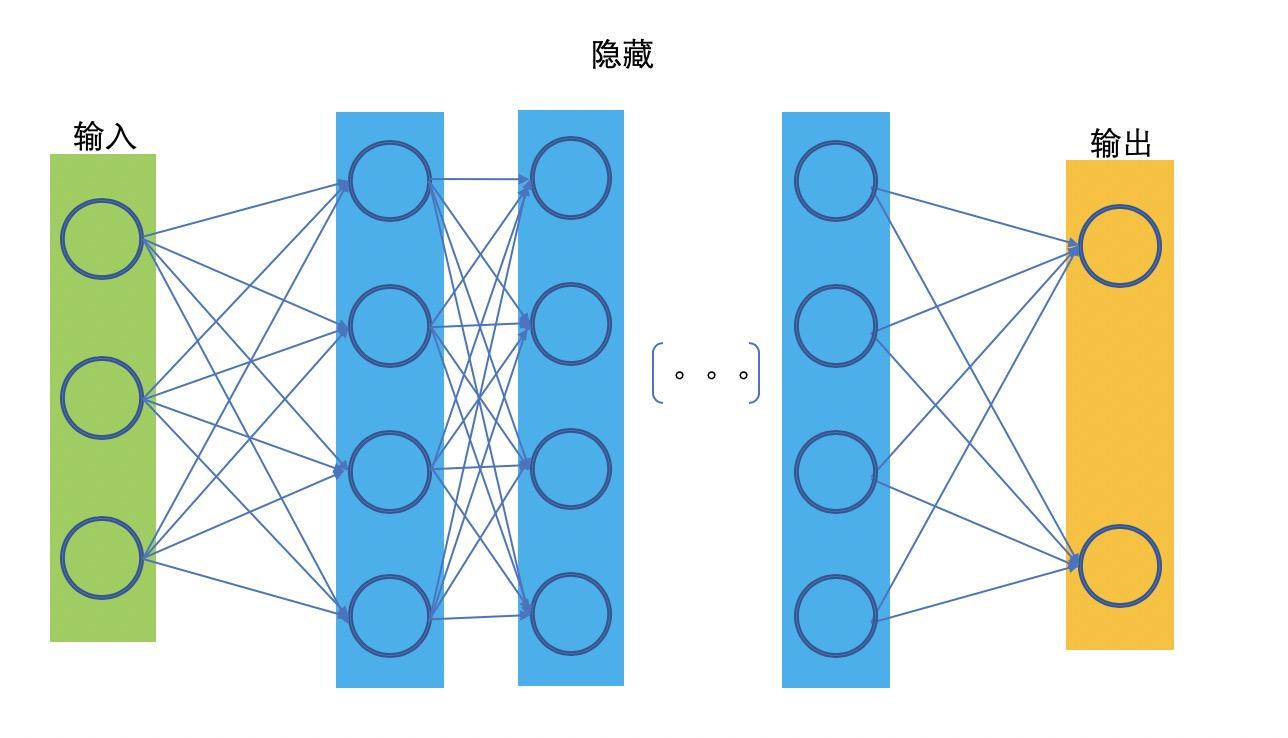
\includegraphics[width=0.65\textwidth]{figture/example.png}
    \caption*{图 1-1 \quad 2005 年相对 2001 年，5 所大学 SCI-e 文献总数增幅图}
\end{figure}

（5）图的大小一般为\textcolor{blue}{宽 6.67 cm $\times$ 高 5.00 cm}。特殊情况下，也可宽 9.00 cm $\times$ 高 6.75 cm，或宽 13.5 cm $\times$ 高 9.00 cm。总之，一篇文章中，同类图片的大小应该一致，编排美观、整齐。

（6）一幅图如有若干幅\textcolor{blue}{分图}，均应编分图号，用\textcolor{blue}{(a), (b), (c)......} 按顺序编排，且各分图的分题注直接列在各自分图的正下方，总题注在所有分图的下方正中，如下图所示：

\begin{figure}[h]
    \centering
    \includegraphics[width=0.85\textwidth]{figture/example2.png}
    \caption*{图 1 \quad M10 燃料对汽油机全负荷速度特性的影响}
\end{figure}

\vfill
\begin{flushleft} 2 \end{flushleft}

\clearpage % ----------------- 分页：进入第19页 -----------------

\fancyhead[C]{\zihao{5} 1 绪论}
\fancyfoot[C]{\zihao{5} 3}

\noindent {\color{red}\textbf{表：}}

（1） 如某个表需要转页接排，在随后的各页上应重复表的编号。编号后跟表题（可省略）和“（续）”，如表 1（续），续表均应重复表头和关于单位的陈述。

表格的设计应紧跟文述。表的编排一般是内容和测试项目由左至右横读，数据依序竖读，应有自明性。若为大表或作为工具使用的表格，可作为附表在附录中给出，论文中的表格参数应标明量和单位的符号；

（2）表中各物理量及量纲均按国际标准(SI) 及国家规定的法定符号和法定计量单位标注；

（3）一律使用三线表，与文字齐宽，{\color{red}顶线和底线线粗 1 $\frac{1}{2}$ 磅}，中线线粗 1 磅。例如表 1-1；

（4）使用他人表格须注明出处。

（5）表中用字为{\color{blue}五号字体}。如排列过密，用五号字有困难时，可小于五号字，但不小于七号。

（6）{\color{magenta}表格必须通栏，即表格宽度与正文版面平齐，如下表所示。}

\begin{table}[htbp]
    \zihao{5}
    \centering
    \caption{文献类型和标志代码}
    \begin{tabularx}{\textwidth}{lclc}
        \toprule
        文献类型 & {\color{blue}标志代码} & 文献类型 & {\color{blue}标志代码} \\
        \midrule
        普通图书 & M & 会议录 & C \\
        汇编 & G & 报纸 & N \\
        期刊 & J & 学位论文 & D \\
        报告 & R & 标准 & S \\
        专利 & P & 数据库 & DB \\
        计算机程序 & CP & 电子公告 & EB \\
        \bottomrule
    \end{tabularx}
\end{table}

\vspace{2em}
在三线表中可以加辅助线，以适应较复杂表格的需要，如表 1-2 所示。

\clearpage % ----------------- 分页：进入第20页 -----------------

\fancyhead[C]{\zihao{5} 西安交通大学博士/硕士学位论文}
\fancyfoot[C]{\zihao{5} 4}

\begin{table}[htbp]
    \zihao{5}
    \centering
    \caption{方弯管内流动最大速度比较}
    \begin{tabularx}{\textwidth}{Xcccc}
        \toprule
        \multirow{2}{*}{项目} & \multicolumn{2}{c}{层流} & \multicolumn{2}{c}{紊流} \\
        \cmidrule(lr){2-3} \cmidrule(lr){4-5}
         & 0$^\circ$截面 & 90$^\circ$截面 & 0$^\circ$截面 & 90$^\circ$截面 \\
        \midrule
        理论值 $V_{\max}$/m$\cdot$s$^{-1}$ & 0.04 & 0.03 & 1.30 & 1.25 \\
        计算值 $V_{\max}$/m$\cdot$s$^{-1}$ & 0.04 & 0.03 & 1.26 & 1.21 \\
        误差/\% & 0.00 & 3.12 & 3.07 & 3.20 \\
        \bottomrule
    \end{tabularx}
\end{table}

\vspace{4em}
\noindent {\color{red}\textbf{公式：}}

（1）公式应另起一行，居中编排，较长的公式尽可能在等号后换行，或者在“+”、“-”等符号后换行。公式中分数线的横线，长短要分清，主要的横线应与等号取平。

（2）公式后应注明编号，公式号应置于小括号中，如公式（2-3）。写在右边行末，中间不加虚线；

（3）公式下面的“式中：”两字左起顶格编排，后接符号及其解释；解释顺序为先左后右，先上后下；解释与解释之间用“；”隔开。

（4）公式中各物理量及量纲均按国际标准（SI）及国家规定的法定符号和法定计量单位标注，禁止使用已废弃的符号和计量单位。

\noindent \textbf{范例：}
\begin{equation}
    q = k_d H^x \label{eq:1-1}
\end{equation}
\noindent {\color{red}式中：}$q$ —— 灌水器流量/L$\cdot$h-1；$k_d$ —— 流量系数；$H$ —— 工作压力/m；$x$ —— 流态指数。

\noindent {\color{red}（此处，“式中：”改为顶格输出）}

\clearpage % ----------------- 分页：进入第21页 -----------------

\fancyhead[C]{\zihao{5} 1 绪论}
\fancyfoot[C]{\zihao{5} 5}

\noindent （1-1）中，（公式引用）..................

\vspace{2em}
\begin{equation}
    \sqrt{b^2-4ac} = \frac{-b \pm \sqrt{b^2-4ac}}{2a} \cdot \frac{n!}{r!(n-r)!} \cdot \frac{-b \pm \sqrt{b^2-4ac}}{2a} \cdot \frac{-b \pm \sqrt{b^2-4ac}}{2a} \label{eq:1-2}
\end{equation}

\vfill

% ============================================================
% 第 2 章 (对应 PDF 22-23 页 / 打印页码 6-7)
% ============================================================
\clearpage
\setcounter{chapter}{1} % 设置章节为 2
\setcounter{page}{6}    % 对应 PDF 第 22 页

% --- 第 22 页 (偶数页) ---
\fancyhead[C]{\zihao{5} 西安交通大学博士/硕士学位论文}
\fancyfoot[C]{\zihao{5} 6}

% 章标题居中，距离页眉横线约1cm
\vspace{1cm}
\begin{center}
    {\zihao{3}\sffamily 2 \quad XX（标题 1）}
\end{center}
\vspace{0.8cm}

% 2.1 标题 2 - 顶格（不缩进）
\noindent {\zihao{4} 2.1 \quad 标题 2}

% 2.1.1 标题 3 - 缩进2em
\vspace{0.3cm}
\noindent \hspace{2em} {\zihao{-4} 2.1.1 \quad 标题 3}

\vspace{1.2cm}

% 正文段落：缩进2em，与2.1.1对齐
\noindent \hspace{2em} 公式按章重新编号：

\vspace{0.6cm}

% 公式编号格式：(2-1)，使用 \tag 手动设置
\begin{equation}
    \frac{n!}{r!(n-r)!} \frac{1}{2} \tag{2-1} \label{eq:2-1}
\end{equation}

\vspace{1.8cm}

% 公式说明：缩进2em
\noindent \hspace{2em} 公式（2-1）说明，…………（公式在正文中的引用）

\vspace{3.5cm}

% 图题注：缩进2em
\noindent \hspace{2em} 图题注：

\vspace{0.8cm}

% 图注：居中
\begin{center}
    \zihao{5} 图 2-1 \quad XXXXXX
\end{center}

% --- 第 23 页 (奇数页：空白页/预留页) ---
\newpage
\fancyhead[C]{\zihao{5} 2 \quad XX（标题 1）}
\fancyfoot[C]{\zihao{5} 7}
\vspace*{5cm}
\begin{center}
    {\color{white} Equation Chapter (Next) Section 1}
\end{center}

% ============================================================
% 第 3 章 (对应 PDF 24-25 页 / 打印页码 8-9)
% ============================================================
\clearpage
\setcounter{chapter}{2} % 第3章
\setcounter{page}{8}    % 页码8

% --- 第 24 页 (偶数页) ---
\fancyhead[C]{\zihao{5} 西安交通大学博士/硕士学位论文}
\fancyfoot[C]{\zihao{5} 8}

% 章标题
\vspace{1cm}
\begin{center}
    {\zihao{3}\sffamily 3 \quad XXX（标题 1）}
\end{center}
\vspace{0.8cm}

% 3.1 标题 2
\noindent{\zihao{4} 3.1 \quad 标题 2}

% 3.1.1 标题 3 （缩进 2em 带 * ✅）
\vspace{0.3cm}
\hspace*{2em}{\zihao{-4} 3.1.1 \quad 标题 3}

\vspace{1.2cm}

% 正文（缩进 2em 带 * ✅）
\hspace*{2em}公式按章重新编号：

\vspace{0.6cm}

% 公式
\begin{equation}
    \frac{n!}{r!(n-r)!} \frac{1}{2} \tag{3-1} \label{eq:3-1}
\end{equation}

\vspace{1.8cm}

% 公式说明
\hspace*{2em}公式（3-1）说明，…………（公式在正文中的引用）

\vspace{3.5cm}

% 图题注
\hspace*{2em}图题注：

\vspace{0.8cm}

% 图注
\begin{center}
    \zihao{5} 图 3-1 \quad XXXXXX
\end{center}

% --- 第 25 页 空白页 ---
\newpage
\fancyhead[C]{\zihao{5} 3 \quad XXX（标题 1）}
\fancyfoot[C]{\zihao{5} 9}
\vfill
\begin{center}
    {\color{white} Equation Chapter (Next) Section 1}
\end{center}
\vfill


% --- 第 4 章 (PDF 26-27 页 / 打印页码 10-11) ---
% ============================================================
% 第 4 章 (对应 PDF 26-27 页 / 打印页码 10-11)
% ============================================================
\clearpage
\setcounter{chapter}{3} % 设置章节为 4
\setcounter{page}{10}    % 对应 PDF 第 26 页

% --- 第 10 页 (偶数页) ---
\fancyhead[C]{\zihao{5} 西安交通大学博士/硕士学位论文}
\fancyfoot[C]{\zihao{5} 10}

% 章标题居中，距离页眉横线约1cm
\vspace{1cm}
\begin{center}
{\zihao{3}\sffamily 4 \quad XXXX（标题 1）}
\end{center}
\vspace{0.8cm}

% 4.1 标题 2 - 顶格（不缩进）
\noindent {\zihao{4} 4.1 \quad 标题 2}

% 4.1.1 标题 3 - 缩进2em
\vspace{0.3cm}
\noindent \hspace{2em} {\zihao{-4} 4.1.1 \quad 标题 3}

\vspace{1.2cm}

% 正文段落：缩进2em
\noindent \hspace{2em} 公式按章重新编号：

\vspace{0.6cm}

% 公式编号格式：(4-1)
\begin{equation}
\frac{n!}{r!(n-r)!} \frac{1}{2} \tag{4-1} \label{eq:4-1}
\end{equation}

\vspace{1.8cm}

% 公式说明：缩进2em
\noindent \hspace{2em} 公式（4-1）说明，…………（公式在正文中的引用）

\vspace{3.5cm}

% 图题注：缩进2em
\noindent \hspace{2em} 图题注：

\vspace{0.8cm}

% 图注：居中
\begin{center}
\zihao{5} 图 4-1 \quad XXXXXX
\end{center}

% --- 第 11 页 (奇数页：空白页/预留页) ---
\newpage
\fancyhead[C]{\zihao{5} 4 \quad XXXX（标题 1）}
\fancyfoot[C]{\zihao{5} 11}
\vspace*{5cm}
\begin{center}
{\color{white} Equation Chapter (Next) Section 1}
\end{center}


% ============================================================
% 第 5 章 (对应 PDF 28-29 页 / 打印页码 12-13)
% ============================================================
\clearpage
\setcounter{chapter}{4} % 设置章节为 5
\setcounter{page}{12}    % 对应 PDF 第 28 页

% --- 第 12 页 (偶数页) ---
\fancyhead[C]{\zihao{5} 西安交通大学博士/硕士学位论文}
\fancyfoot[C]{\zihao{5} 12}

% 章标题居中，距离页眉横线约1cm
\vspace{1cm}
\begin{center}
{\zihao{3}\sffamily 5 \quad XXXXX（标题 1）}
\end{center}
\vspace{0.8cm}

% 5.1 标题 2 - 顶格
\noindent {\zihao{4} 5.1 \quad 标题 2}

% 5.1.1 标题 3 - 缩进2em
\vspace{0.3cm}
\noindent \hspace{2em} {\zihao{-4} 5.1.1 \quad 标题 3}

\vspace{1.2cm}

% 正文段落：缩进2em
\noindent \hspace{2em} 公式按章重新编号：

\vspace{0.6cm}

% 公式编号格式：(5-1)
\begin{equation}
\frac{n!}{r!(n-r)!} \frac{1}{2} \tag{5-1} \label{eq:5-1}
\end{equation}

\vspace{1.8cm}

% 公式说明：缩进2em
\noindent \hspace{2em} 公式（5-1）说明，…………（公式在正文中的引用）

\vspace{3.5cm}

% 图题注：缩进2em
\noindent \hspace{2em} 图题注：

\vspace{0.8cm}

% 图注：居中
\begin{center}
\zihao{5} 图 5-1 \quad XXXXXX
\end{center}

% --- 第 13 页 (奇数页：空白页/预留页) ---
\newpage
\fancyhead[C]{\zihao{5} 5 \quad XXXXX（标题 1）}
\fancyfoot[C]{\zihao{5} 13}
\vspace*{5cm}
\begin{center}
{\color{white} Equation Chapter (Next) Section 1}
\end{center}
%P6
% ============================================================
% 第 6 章 (对应 PDF 30-31 页 / 打印页码 14-15)
% ============================================================
\clearpage
\setcounter{chapter}{5} 
\setcounter{page}{14}    

% --- 第 14 页 (偶数页) ---
\fancyhead[C]{\zihao{5} 西安交通大学博士/硕士学位论文}
\fancyfoot[C]{\zihao{5} 14}

\vspace{1cm}
\begin{center}
{\zihao{3}\sffamily 6 \quad XXXXXX（标题 1）}
\end{center}
\vspace{0.8cm}

\noindent {\zihao{4} 6.1 \quad 标题 2}

\vspace{0.3cm}
\noindent \hspace{2em} {\zihao{-4} 6.1.1 \quad 标题 3}

\vspace{1.2cm}
\noindent \hspace{2em} 公式按章重新编号：
\vspace{0.6cm}
\begin{equation}
\frac{n!}{r!(n-r)!} \frac{1}{2} \tag{6-1} \label{eq:6-1}
\end{equation}

\vspace{1.8cm}
\noindent \hspace{2em} 公式（6-1）说明，…………（公式在正文中的引用）
\vspace{3.5cm}

% 图题注：缩进2em
\noindent \hspace{2em} 图题注：

\vspace{0.8cm}

% 图注：居中
\begin{center}
    \zihao{5} 图 6-1 \quad XXXXXX
\end{center}

% --- 第 15 页 (奇数页：空白预留页) ---
\newpage
\fancyhead[C]{\zihao{5} 6 \quad XXXXXX（标题 1）}
\fancyfoot[C]{\zihao{5} 15}
\vspace*{5cm}
\begin{center}
{\color{white} Equation Chapter (Next) Section 1}
\end{center}


% ============================================================
% 第 7 章 (对应 PDF 32 页 / 打印页码 16)
% ============================================================
\clearpage
\setcounter{chapter}{6}
\setcounter{page}{16}

% --- 第 16 页 (偶数页) ---
\fancyhead[C]{\zihao{5} 西安交通大学博士/硕士学位论文}
\fancyfoot[C]{\zihao{5} 16}

\vspace{1cm}
\begin{center}
{\zihao{3}\sffamily 7 \quad XXXXXXX（标题 1）}
\end{center}
\vspace{0.8cm}

\noindent {\zihao{4} 7.1 \quad 标题 2}

\vspace{0.3cm}
\noindent \hspace{2em} {\zihao{-4} 7.1.1 \quad 标题 3}

\vspace{1.2cm}
\noindent \hspace{2em} 公式按章重新编号：
\vspace{0.6cm}
\begin{equation}
\frac{n!}{r!(n-r)!} \frac{1}{2} \tag{7-1} \label{eq:7-1}
\end{equation}

\vspace{1.8cm}
\noindent \hspace{2em} 公式（7-1）说明，…………（公式在正文中的引用）
\vspace{3.5cm}

% 图题注：缩进2em
\noindent \hspace{2em} 图题注：

\vspace{0.8cm}

% 图注：居中
\begin{center}
    \zihao{5} 图 7-1 \quad XXXXXX
\end{center}
\vfill
\begin{center} {\color{white} Equation Chapter (Next) Section 1} \end{center}


% ============================================================
% 第 8 章 (对应 PDF 33-34 页 / 打印页码 17-18)
% ============================================================
\clearpage
\setcounter{chapter}{7}
\setcounter{page}{17}

% --- 第 17 页 (奇数页) ---
\fancyhead[C]{\zihao{5} 8 \quad XXXXXXXX（标题 1）}
\fancyfoot[C]{\zihao{5} 17}

\vspace{1cm}
\begin{center}
{\zihao{3}\sffamily 8 \quad XXXXXXXX（标题 1）}
\end{center}
\vspace{0.8cm}

\noindent {\zihao{4} 8.1 \quad 标题 2}

\vspace{0.3cm}
\noindent \hspace{2em} {\zihao{-4} 8.1.1 \quad 标题 3}

\vspace{1.2cm}
\noindent \hspace{2em} 公式按章重新编号：
\vspace{0.6cm}
\begin{equation}
\frac{n!}{r!(n-r)!} \frac{1}{2} \tag{8-1} \label{eq:8-1}
\end{equation}

\vspace{1.8cm}
\noindent \hspace{2em} 公式（8-1）说明，…………（公式在正文中的引用）
\vspace{3.5cm}

% 图题注：缩进2em
\noindent \hspace{2em} 图题注：

\vspace{0.8cm}

% 图注：居中
\begin{center}
    \zihao{5} 图 8-1 \quad XXXXXX
\end{center}

% --- 第 18 页 (偶数页：空白预留页) ---
\newpage
\fancyhead[C]{\zihao{5} 西安交通大学博士/硕士学位论文}
\fancyfoot[C]{\zihao{5} 18}
\vspace*{5cm}
\begin{center}
{\color{white} Equation Chapter (Next) Section 1}
\end{center}


% ============================================================
% 第 9 章 (对应 PDF 35-36 页 / 打印页码 19-20)
% ============================================================
\clearpage
\setcounter{chapter}{8}
\setcounter{page}{19}

% --- 第 19 页 (奇数页) ---
\fancyhead[C]{\zihao{5} 9 \quad XXXXXXXXX（标题 1）}
\fancyfoot[C]{\zihao{5} 19}

\vspace{1cm}
\begin{center}
{\zihao{3}\sffamily 9 \quad XXXXXXXXX（标题 1）}
\end{center}
\vspace{0.8cm}

\noindent {\zihao{4} 9.1 \quad 标题 2}

\vspace{0.3cm}
\noindent \hspace{2em} {\zihao{-4} 9.1.1 \quad 标题 3}

\vspace{1.2cm}
\noindent \hspace{2em} 公式按章重新编号：
\vspace{0.6cm}
\begin{equation}
\frac{n!}{r!(n-r)!} \frac{1}{2} \tag{9-1} \label{eq:9-1}
\end{equation}

\vspace{1.8cm}
\noindent \hspace{2em} 公式（9-1）说明，…………（公式在正文中的引用）
\vspace{3.5cm}

% 图题注：缩进2em
\noindent \hspace{2em} 图题注：

\vspace{0.8cm}

% 图注：居中
\begin{center}
    \zihao{5} 图 9-1 \quad XXXXXX
\end{center}

% --- 第 20 页 (偶数页：空白预留页) ---
\newpage
\fancyhead[C]{\zihao{5} 西安交通大学博士/硕士学位论文}
\fancyfoot[C]{\zihao{5} 20}
\vspace*{5cm}
\begin{center}
{\color{white} Equation Chapter (Next) Section 1}
\end{center}


% ============================================================
% 第 10 章 (对应 PDF 37-38 页 / 打印页码 21-22)
% ============================================================
\clearpage
\setcounter{chapter}{9}
\setcounter{page}{21}

% --- 第 21 页 (奇数页) ---
\fancyhead[C]{\zihao{5} 10 \quad XXXXXXXXXX（标题 1）}
\fancyfoot[C]{\zihao{5} 21}

\vspace{1cm}
\begin{center}
{\zihao{3}\sffamily 10 \quad XXXXXXXXXX（标题 1）}
\end{center}
\vspace{0.8cm}

\noindent {\zihao{4} 10.1 \quad 标题 2}

\vspace{0.3cm}
\noindent \hspace{2em} {\zihao{-4} 10.1.1 \quad 标题 3}

\vspace{1.2cm}
\noindent \hspace{2em} 公式按章重新编号：
\vspace{0.6cm}
\begin{equation}
\frac{n!}{r!(n-r)!} \frac{1}{2} \tag{10-1} \label{eq:10-1}
\end{equation}

\vspace{1.8cm}
\noindent \hspace{2em} 公式（10-1）说明，…………（公式在正文中的引用）
\vspace{3.5cm}

% 图题注：缩进2em
\noindent \hspace{2em} 图题注：

\vspace{0.8cm}

% 图注：居中
\begin{center}
    \zihao{5} 图 10-1 \quad XXXXXX
\end{center}

% --- 第 22 页 (偶数页：空白预留页) ---
\newpage
\fancyhead[C]{\zihao{5} 西安交通大学博士/硕士学位论文}
\fancyfoot[C]{\zihao{5} 22}
\vspace*{5cm}
\begin{center}
{\color{white} Equation Chapter (Next) Section 1}
\end{center}


% ============================================================
% 第 11 章 (对应 PDF 39-40 页 / 打印页码 23-24)
% ============================================================
\clearpage
\setcounter{chapter}{10}
\setcounter{page}{23}

% --- 第 23 页 (奇数页) ---
\fancyhead[C]{\zihao{5} 11 \quad XXXXXXXXXXX（标题 1）}
\fancyfoot[C]{\zihao{5} 23}

\vspace{1cm}
\begin{center}
{\zihao{3}\sffamily 11 \quad XXXXXXXXXXX（标题 1）}
\end{center}
\vspace{0.8cm}

\noindent {\zihao{4} 11.1 \quad 标题 2}

\vspace{0.3cm}
\noindent \hspace{2em} {\zihao{-4} 11.1.1 \quad 标题 3}

\vspace{1.2cm}
\noindent \hspace{2em} 公式按章重新编号：
\vspace{0.6cm}
\begin{equation}
\frac{n!}{r!(n-r)!} \frac{1}{2} \tag{11-1} \label{eq:11-1}
\end{equation}

\vspace{1.8cm}
\noindent \hspace{2em} 公式（11-1）说明，…………（公式在正文中的引用）
\vspace{3.5cm}

% 图题注：缩进2em
\noindent \hspace{2em} 图题注：

\vspace{0.8cm}

% 图注：居中
\begin{center}
    \zihao{5} 图 11-1 \quad XXXXXX
\end{center}

% --- 第 24 页 (偶数页：空白预留页) ---
\newpage
\fancyhead[C]{\zihao{5} 西安交通大学博士/硕士学位论文}
\fancyfoot[C]{\zihao{5} 24}
\vspace*{5cm}
\begin{center}
{\color{white} Equation Chapter (Next) Section 1}
\end{center}

% ============================================================
% 第 12 章 结论与展望 (对应 PDF 41-42 页 / 打印页码 25-26)
% ============================================================
\clearpage
\setcounter{chapter}{11} % 设置章节为 12
\setcounter{page}{25}    % 对应 PDF 第 41 页

% --- 第 25 页 (奇数页) ---
\fancyhead[C]{\zihao{5} 12 \quad 结论与展望}
\fancyfoot[C]{\zihao{5} 25}

% 章标题居中，距离页眉横线约1cm
\vspace{1cm}
\begin{center}
    {\zihao{3}\sffamily 12 \quad 结论与展望}
\end{center}
\vspace{0.8cm}

% 结论说明文字（缩进2em，与正文对齐）
\noindent \hspace{2em} 结论部分着重总结出论文的创新点或新见解及研究展望或建议。

\vspace{0.8cm}

% 12.1 标题 2 - 顶格（不缩进）
\noindent {\zihao{4} 12.1 \quad 标题 2}

% 12.1.1 标题 3 - 缩进2em
\vspace{0.3cm}
\noindent \hspace{2em} {\zihao{-4} 12.1.1 \quad 标题 3}

\vspace{1.2cm}

% 正文段落：缩进2em，与12.1.1对齐
\noindent \hspace{2em} 公式按章重新编号：

\vspace{0.6cm}

% 公式编号格式：(12-1)，使用 \tag 手动设置
\begin{equation}
    \frac{n!}{r!(n-r)!} \frac{1}{2} \tag{12-1} \label{eq:12-1}
\end{equation}

\vspace{1.8cm}

% 公式说明：缩进2em
\noindent \hspace{2em} 公式（12-1）说明，…………（公式在正文中的引用）

\vspace{3.5cm}

% 图题注：缩进2em
\noindent \hspace{2em} 图题注：

\vspace{0.8cm}

% 图注：居中
\begin{center}
    \zihao{5} 图 12-1 \quad XXXXXX
\end{center}

% --- 第 26 页 (偶数页：空白页/预留页) ---
\newpage
\fancyhead[C]{\zihao{5} 西安交通大学博士/硕士学位论文}
\fancyfoot[C]{\zihao{5} 26}
\vspace*{5cm}
\begin{center}
    {\color{white} Equation Chapter (Next) Section 1}
\end{center}
% 后置部分
% ------------------------------------------------------------
\backmatter
\pagestyle{backmatterstyle}

% ------------------------------------------------------------
% 第27页：致谢
% ------------------------------------------------------------

% 致谢页页眉显示前一章标题（单线）
\pagestyle{fancy}
\fancyhf{}
\fancyhead[C]{\zihao{5} 12 \quad 结论与展望}
\fancyfoot[C]{\thepage}
\renewcommand{\headrulewidth}{0.4pt}

% 标题居中，距离双横线约1cm
\vspace*{0.3cm}
\begin{center}
    {\zihao{3}\sffamily 致\quad 谢}
\end{center}
\addcontentsline{toc}{chapter}{致谢}
\vspace{0.5cm}

{\zihao{-4}
致谢中主要感谢导师和对论文工作有直接贡献和帮助的人士和单位。

一般致谢的内容有：

（一）对指导或协助指导完成论文的导师；

（二）对国家科学基金、资助研究工作的奖学金基金、合同单位、资助或支持的企业、组织或个人；

（三）对协助完成研究工作和提供便利条件的组织或个人；

（四）对在研究工作中提出建议和提供帮助的人；

（五）对给予转载和引用权的资料、图片、文献、研究思想和设想的所有者；

（六）对其他应感谢的组织和个人。

致谢言语应谦虚诚恳，实事求是。字数不超过 1000 汉字

\vspace{2cm}

\noindent {\color{red}用于双盲评审的论文，此页内容全部隐去。}
}

% ------------------------------------------------------------
% ------------------------------------------------------------
% 导言区需确认加载：\usepackage{xcolor, tabularx, booktabs, setspace}
% ------------------------------------------------------------

% ============================================================
% 第 28 页 (PDF 第 44 页)：参考文献第一页
% ============================================================
\clearpage
\pagestyle{fancy}
\fancyhf{}
\fancyhead[C]{\zihao{5} 西安交通大学博士/硕士学位论文}
\fancyfoot[C]{\thepage}
\renewcommand{\headrulewidth}{0.4pt}
\setcounter{page}{28}

% 标题紧贴页眉双横线下方一行，居中，不加粗
\vspace*{0.3cm}
\begin{center}
    {\zihao{3}\sffamily 参考文献}
\end{center}
\addcontentsline{toc}{chapter}{参考文献}
\vspace{0.3cm}

% 红色提示文字（标红加粗）
\noindent {\color{red}\bfseries （此上两空行不能删除，是为 EndNote 的参考文献列表所预留）}

\begin{spacing}{1.5}
\zihao{-4}

% 第一段：缩进2em
\noindent \hspace{2em}文后著录的参考文献务必实事求是。论文中引用过的文献必须著录，未引用的文献不得出现。应遵循学术道德规范，避免涉嫌抄袭、剽窃等学术不端行为。

\vspace{0.3cm}
% 第二段：缩进2em
\noindent \hspace{2em}参考文献一般应是作者亲自考察过的对学位论文有参考价值的文献，除特殊情况外，一般不应间接引用。

\vspace{0.3cm}
% 第三段：缩进2em
\noindent \hspace{2em}参考文献应有权威性，要注意引用最新的文献。

\vspace{0.3cm}
% 第四段：缩进2em
\noindent \hspace{2em}参考文献的数量：

\vspace{0.3cm}
% 第五段：缩进2em，蓝色文字
\noindent \hspace{2em}博士学位论文，一般应在 {\color{blue}80 篇以上}，其中，{\color{blue}期刊文献 60 篇以上，国外文献 30 篇以上，均以近 5 年的文献为主}。

\vspace{0.3cm}
% 第六段：缩进2em，蓝色文字
\noindent \hspace{2em}硕士学位论文，一般应在 {\color{blue}30 篇以上}，其中，{\color{blue}期刊文献不少于 20 篇，国外文献不少于 10 篇，均以近 5 年的文献为主}。

\vspace{0.3cm}
% 第七段：缩进2em
\noindent \hspace{2em}对于申请专业学位的学位论文，参考文献的数量可参照执行。

\vspace{0.3cm}
% 第八段：缩进2em
\noindent \hspace{2em}参考文献的著录格式应符合国家标准 GB/T 7714-2015《文后参考文献著录规则》。参考文献中每条项目应齐全。
\end{spacing}


% ============================================================
% 第 29 页 (PDF 第 45 页)
% ============================================================
\clearpage
\thispagestyle{refdoublelinestyle}
\pagestyle{refdoublelinestyle}

\begin{spacing}{1.5}
\zihao{-4}

\vspace{0.3cm}
\noindent \textbf{1. 顺序编码制}

\vspace{0.3cm}
\noindent 文献中的作者不超过三位时全部列出，超过三位时，一般{\color{blue}只列前三位}，中文的后面加 {\color{blue}“，等”}字，英文的后面加 {\color{blue}“, et al”}，作者姓名之间用{\color{blue}逗号}分开。

\vspace{0.3cm}
\noindent 外国人名一般采用{\color{blue}姓在前，名在后}的著录法，{\color{blue}姓全写且第一个字母大写，名简写成单个大写字母且不加标点}，姓和名之间空 1 格，如：“{\color{blue}Metcalf S W}”。也可采用名在前，姓在后的著录法，姓全写且第一个字母大写，名简写成单个大写字母且不加标点，名和姓之间空 1 格，如：“{\color{blue}S W Metcalf}”。

\vspace{0.3cm}
\noindent 中文人名的英文表达方式：

\vspace{0.3cm}
\noindent 简写时，采用{\color{blue}姓在前，名在后}的著录法，{\color{blue}姓全写且第一个字母大写，名简写成单个大写字母且不加标点}，如，“钱学森”，简写为“{\color{blue}Qian XS}”。

\vspace{0.3cm}
\noindent 全拼时，{\color{blue}名在前，姓在后}的著录法，名的第一个字母大写，名连写，名后空 1 格写姓，姓的第一个字母大写。如，“钱学森”，写为“{\color{blue}Xuesen Qian}”。

\vspace{0.3cm}
\noindent 文后参考文献著录格式{\color{blue}范例样板}，采用五号。
\end{spacing}


% ============================================================
% 第 30 页 (PDF 第 46 页)
% ============================================================
\clearpage
\thispagestyle{refdoublelinestyle}
\pagestyle{refdoublelinestyle}

% 确保页眉正确显示
\fancyhf{}
\fancyhead[C]{\zihao{5}西安交通大学博士/硕士学位论文}
\fancyfoot[C]{}
\renewcommand{\headrulewidth}{0.4pt}
\renewcommand{\headrule}{%
    \hrule width\headwidth height\headrulewidth\vskip 2pt%
    \hrule width\headwidth height\headrulewidth%
}

\begin{spacing}{1.5}
\zihao{-4}

\vspace{0.3cm}
\noindent \textbf{具体要求如下：}

\vspace{0.3cm}
\noindent \textbf{A 专著}（包括普通图书［M］、论文集和会议录［C］、科技报告［R］、学位论文［D］、标准［S］）

\vspace{0.3cm}
\noindent 主要责任者．文献题名［文献类型标志］．其他责任者．{\color{magenta}版本项(第 1 版不标注)} ．出版地：出版者，出版年：引文页码．获取和访问路径．

\vspace{0.3cm}
\noindent \textbf{B 专著中的析出文献}

\vspace{0.3cm}
\noindent 析出文献主要责任者．析出文献题名[文献类型标志]．析出文献其他责任者//专著主要责任者．专著题名：其他题名信息. {\color{magenta}版本项(第 1 版不标注)} ．出版地：出版者，出版年：析出文献的起止页码．获取和访问路径．

\vspace{0.3cm}
\noindent \textbf{C 连续出版物}

\vspace{0.3cm}
\noindent 主要责任者．题名:其他题名信息［文献类型标志］．年，卷（期）－年，卷（期）. 出版地：出版者，出版年．获取和访问路径．

\vspace{0.3cm}
\noindent \textbf{D 连续出版物中的析出文献}（包括期刊中析出的文献[J]、报纸中析出的文献[N].）

\vspace{0.3cm}
\noindent 析出文献主要责任者．析出文献题名［文献类型标志］．连续出版物题名：其他题名信息，年，卷（期）：页码．获取和访问路径．

\vspace{0.3cm}
\noindent \textbf{E 专利文献}

\vspace{0.3cm}
\noindent 专利发明者/专利申请者或所有者．专利题名: 专利国别,专利号［文献类型标志］. 公告日期或公开日期. 获取和访问路径．

\vspace{0.3cm}
\noindent \textbf{F 电子文献}（包括专著或连续出版物中析出的电子文献）

\vspace{0.3cm}
\noindent 主要责任者．题名：其他题名信息[文献类型标志/载体类型标志]．出版地：出版者，出版年（更新或修改日期）［引用日期］．获取和访问路径．
\end{spacing}

\vspace{0.5cm}
\begin{center}
\zihao{5} 表 2-2 \quad 文献类型和标志代码

\vspace{0.3cm}
\begin{tabular}{p{3cm}cp{3cm}c}
\toprule
文献类型 & {\color{blue}标志代码} & 文献类型 & {\color{blue}标志代码} \\
\midrule
普通图书 & {\color{blue}M} & 会议录 & {\color{blue}C} \\
汇编 & {\color{blue}G} & 报纸 & {\color{blue}N} \\
期刊 & {\color{blue}J} & 学位论文 & {\color{blue}D} \\
报告 & {\color{blue}R} & 标准 & {\color{blue}S} \\
专利 & {\color{blue}P} & 数据库 & {\color{blue}DB} \\
计算机程序 & {\color{blue}CP} & 电子公告 & {\color{blue}EB} \\
\bottomrule
\end{tabular}

\vspace{0.5cm}
表 2-3 \quad 电子文献载体和标志代码

\vspace{0.3cm}
\begin{tabular}{p{4cm}cp{4cm}c}
\toprule
载体类型 & {\color{blue}标志代码} & 载体类型 & {\color{blue}标志代码} \\
\midrule
磁带（magnetic tape） & {\color{blue}MT} & 磁盘（disk） & {\color{blue}DK} \\
光盘（CD-ROM） & {\color{blue}CD} & 联机网络（online） & {\color{blue}OL} \\
\bottomrule
\end{tabular}
\end{center}


% ============================================================
% 第 31 页 (PDF 第 47 页)
% ============================================================
\clearpage
\pagestyle{fancy}
\fancyhf{}
\fancyhead[C]{\zihao{5} 西安交通大学博士/硕士学位论文}
\renewcommand{\headrulewidth}{0.4pt}
\renewcommand{\headrule}{%
    \hrule width\headwidth height\headrulewidth\vskip 2pt%
    \hrule width\headwidth height\headrulewidth%
}
\fancyfoot[C]{}

% 标题紧贴页眉双横线下方一行，居中，不加粗
\vspace*{0.3cm}
\begin{center}
    {\zihao{3}\sffamily 参考文献}
\end{center}
\vspace{0.3cm}

\noindent \zihao{-4}\textbf{样例：}

\vspace{0.3cm}
\zihao{5}
\begin{spacing}{1.3}
\noindent [1] 刘国钧，郑如斯．中国书的故事［M］．北京：中国青年出版社，1979：110-115．

\vspace{0.2cm}
\noindent [2] 昂温 G．外国出版史［M］．陈生铮译．北京：中国书籍出版社，1988．

\vspace{0.2cm}
\noindent [3] 辛希孟．信息技术与信息服务国际研讨会论文集：A 集［C］．北京：中国社会科学出版社，1979．

\vspace{0.2cm}
\noindent [4] 冯西桥．核反应堆压力容器的 LBB 分析［R］．北京：核能技术设计研究院，1997．

\vspace{0.2cm}
\noindent [5] 张和生．地质力学系统理论［D］．太原：太原理工大学，1998．

\vspace{0.2cm}
\noindent [6] 全国文献工作标准化技术委员会第七分委员会．GB/T 5795-1986．中国标准书号［S］．北京：中国标准出版社，1986．

\vspace{0.2cm}
\noindent [7] 罗云．安全科学理论体系的发展及趋势探讨［M］//白春华，何学秋，吴宗之．21世纪安全科学与技术的发展趋势．北京：科学出版社，2000：1-5．

\vspace{0.2cm}
\noindent [8] 钟文发．非线性规划在可燃毒物配置中的应用［C］//赵玮．运筹学的理论与应用：中国运筹学会第五届大会论文集．西安：西安电子科技大学出版社，1996：468－471．

\vspace{0.2cm}
\noindent [9] 高义民，张凤华，邢建东等．颗粒增强不锈钢基复合材料冲蚀磨损性能研究［J］．西安交通大学学报，2001，35(7)：727-730．

\vspace{0.2cm}
\noindent [10] Papworth A, Fox P, Zeng GT, et al. Ability of aluminum alloy to wet alumina fibres by addition of bismuth[J]. Mater Sci \& Technol,1999,15(4):419-428.

\vspace{0.2cm}
\noindent [11] 丁文祥．数字革命与竞争国际化［N］．中国青年报，2000－11－20(15)．

\vspace{0.2cm}
\noindent [12] 姜锡洲．一种温热外敷药制备方案：中国，88105607.3［P］．1989-07-26．

\vspace{0.2cm}
\noindent [13] Koseki A, Momose H, Kawahito M, et al. Compiler: US, 828402［P/OL］. 2002-05-25[2002-05-28]. http://FF\&p.

\vspace{0.2cm}
\noindent [14] Online Computer Library Center, Inc. History of OCLC[EB/OL]. [2000-01-08]. http://www.oclc.org/about/history/default.htm.

\vspace{0.2cm}
\noindent [15] 江向东．互联网环境下的信息处理与图书管理系统解决方案［J/OL］．情报学报，1999，18(2)：4[2000-01-18]. http://www.chinainfo.gov.cn/periodical/qbxb.

\vspace{0.2cm}
\noindent [16] Scitor C. Project scheduler[CP/DK]. Sunnyvale,Calif.:Scitor Corp, 1983.

\vspace{0.2cm}
\noindent [17] Metcalf SW. The Tort Hall air emission study[C/OL]//The International Congress on Hazardous Waste, MarquisHotel, Atlanta,Georgia,June 5-8,1995: impact on human and ecological health[1998-09-22]. http://atsdrl.atsdr.cdc.gov:8080/cong95.html.
\end{spacing}

\vspace{0.5cm}
\noindent \zihao{-4}\textbf{2. 著者-出版年制}

\begin{spacing}{1.5}
\zihao{-4}

\vspace{0.3cm}
\noindent A. 正文引用的文献采用著者-出版年制时，各篇文献的标注内容由著者姓氏与出版年构成，并置于“（ ）”内，倘若只标注著者姓氏无法识别该人名时，可标著者姓名，例如中国人、韩国人、日本人用汉字书写姓名。集体著者著述的文献可标注机关团体名称。倘若正文中已提及著者姓名，则在其后的“（ ）”内只著录出版年。

\vspace{0.3cm}
\noindent B. 正文中引用多著者文献时，对欧美著者只需标注第一个著者的姓，其后附“{\color{blue}et al.}”“等”之间留适当空隙。

\vspace{0.3cm}
\noindent C. 在参考文献表中著录同一著者在同一年出版的多篇文献时，出版年后应用小写字母 a, b, c ...区别。

\vspace{0.3cm}
\noindent D. 多次引用同一著者的同一文献，在正文中标注著者与出版年，并在“（ ）”外以角标的形式著录引文页码。

\vspace{0.5cm}
\noindent \textbf{样例：}

\vspace{0.3cm}
\noindent BAKER S K, JACKSON M E. 1995. The future of resource sharing [M]. New York: The Haworth Press.

\vspace{0.3cm}
\noindent 尼葛洛庞帝．1996. 数字化生存［M］．胡永，范海燕，译. 海口：海南出版社．

\vspace{0.3cm}
\noindent 杨宗英．1996. 电子图书馆的现实模型［M］．中国图书馆学报(2): 24-29．

\vspace{0.3cm}
\noindent 刘斌．2014. 力学［M］．合肥：中国科学技术大学出版社．
\end{spacing}


% ============================================================
% 第 32 页 (PDF 第 48 页)：参考文献最后一页
% ============================================================
\clearpage
\thispagestyle{refdoublelinestyle}
\pagestyle{refdoublelinestyle}

% 红色提示文字与上方内容距离3cm，标红加粗
\vspace*{3cm}
\noindent {\zihao{-4}\color{red}\bfseries 参考文献里面标点符号：英文文献用半角,中文文献用全角。}

\vfill
% ------------------------------------------------------------
% 附录页排版
% ------------------------------------------------------------
\clearpage
\setcounter{page}{33} % 设置起始页码为 33

% --- 定义附录页特有的页眉页脚样式 (双线) ---
\fancypagestyle{appendixstyle}{
    \fancyhf{}
    \fancyhead[C]{\zihao{5} 附\quad 录} % 页眉文字
    \fancyfoot[R]{\zihao{5} \thepage}   % 页码位于右下角

    % 双横线
    \renewcommand{\headrulewidth}{0.4pt}
    \renewcommand{\headrule}{%
        \hrule width\headwidth height\headrulewidth\vskip 2pt%
        \hrule width\headwidth height\headrulewidth%
    }
}

\thispagestyle{appendixstyle}
\pagestyle{appendixstyle}

% --- 引入附录内容 ---
% ============================================================
% 附录
% ============================================================

\chapter{附录A}

附录内容示例。

\section{补充表格}

\begin{table}[htbp]
    \centering
    \bicaption{附录数据表}{Appendix Data Table}
    \begin{tabular}{cc}
        \toprule
        \textbf{参数} & \textbf{值} \\
        \midrule
        学习率 & 0.001 \\
        批次大小 & 32 \\
        \bottomrule
    \end{tabular}
\end{table}


\vfill % 自动吸收剩余空间

% ------------------------------------------------------------
% ------------------------------------------------------------
% 第 34 页：攻读学位期间取得的研究成果
% ------------------------------------------------------------
\clearpage
\pagenumbering{arabic}
\setcounter{page}{34} % 设定页码为 34

% --- 1. 页眉页脚设置 ---
\pagestyle{fancy}
\fancyhf{}
\fancyhead[C]{\zihao{5} 西安交通大学博士/硕士学位论文}
\fancyfoot[L]{\zihao{5} 34} % 页码在左下角
\renewcommand{\headrulewidth}{0.75pt}

% --- 2. 章节标题 (三号, 加粗, 居中) ---
\vspace*{0.2cm} % 紧贴横线
\begin{center}
    {\zihao{3}\sffamily\bfseries 攻读学位期间取得的研究成果}
\end{center}
\vspace{0.6cm}

% --- 3. 成果要求列表 (小四号, 1.5倍行距) ---
\begin{spacing}{1.5}
\zihao{-4}
\noindent 1）已发表或已录用的学术论文、已出版的专著/译著、已获授权的专利按参考文献格式列出。

\noindent 2）科研获奖，列出格式为：

\noindent 获奖人（排名情况）．项目名称．奖项名称及等级，发奖机构，获奖时间．

\noindent 3）与学位论文相关的其它成果参照参考文献格式列出。

\noindent 4）全部研究成果连续编号编排。
\end{spacing}

\vspace{1.5cm}

% --- 4. 样例部分 (五号字) ---
\noindent \zihao{5} 样例：

\begin{spacing}{1.2}
\zihao{5}
\noindent [1]\quad Wei ZY, Tang YP, Zhao WH, et al. Rapid development technique for drip irrigation emitters[J]. RP Journal,UK., 2003, 9(2):104~110 (SCI: 000350930600051; EI: 03187452127).

\noindent [2]\quad 魏正英,唐一平,卢秉恒.滴灌管内嵌管状滴头的快速制造方法研究[J].农业工程学报, 2001,17(2):55~58 (EI:01226526279,01416684777).

\noindent [3]\quad 姜锡洲.一种温热外敷药制备方案:中国,88105607.3[P].1989-07-26.

\noindent [4]
\end{spacing}

\vspace{0.3cm}

% --- 5. 蓝色提示说明框 ---
\noindent\begin{minipage}{\textwidth}
\begin{center}
\begin{tcolorbox}[
    colback=white,
    colframe=blue,
    boxrule=1.5pt,
    sharp corners,
    width=0.85\textwidth,
    center,
    halign=center,
    top=2mm, bottom=2mm
]
    % 红底白字的"说明"标签
    \setlength{\fboxsep}{2pt}
    \colorbox{red}{\textcolor{white}{\zihao{4}\bfseries 说明}} \\[2mm]
    
    % 蓝色提示正文
    {\color{blue}\zihao{-4}\bfseries 
    用于双盲评审的论文，只列出已发表的学术论文的篇名、发表刊物名称，\\
    必须隐去各类论文检索号、期号、卷号、页码；专利号；日期等。} \\[2mm]
    
    % 红色删除提醒
    {\color{red}\zihao{3}\bfseries 阅后删除此框及内容。}
\end{tcolorbox}
\end{center}
\end{minipage}

\vfill
% ------------------------------------------------------------
% 第35页/37页：答辩委员会决议 (1:1 复刻版)
% ------------------------------------------------------------
\clearpage
\setcounter{page}{35} % 根据您的截图，页码设为35

% --- 定义页眉双线样式 ---
\fancypagestyle{resolutionstyle}{
    \fancyhf{}
    \fancyhead[C]{\zihao{5}答辩委员会会议决议}
    \fancyfoot[C]{\zihao{5}\thepage}
    \renewcommand{\headrulewidth}{0.4pt}
    \renewcommand{\headrule}{%
        \hrule width\headwidth height\headrulewidth\vskip 2pt%
        \hrule width\headwidth height\headrulewidth%
    }
}
\thispagestyle{resolutionstyle}
\pagestyle{resolutionstyle}

% --- 全局段落与字号设置 ---
\zihao{-4} % 正文小四
\setlength{\parindent}{2em} % 全局首行缩进两个字符
\setstretch{1.4} % 略微收紧行距，确保单页容纳

% --- 标题：三号，居中 ---
\begin{center}
    \vspace*{0.2cm}
    {\zihao{3}\sffamily\bfseries 答辩委员会会议决议}
\end{center}
\addcontentsline{toc}{chapter}{答辩委员会会议决议}

\vspace{0.3cm}

% --- 第一段：缩进 ---
论文提出了

\vspace{3\baselineskip} % 此处精准空出三个物理行

% --- 第二段：缩进，且下方紧跟列表无空行 ---
论文取得的主要创新性成果包括：\nopagebreak % 禁止在此处分页
\begin{enumerate}[leftmargin=4.5em, labelsep=0.5em, topsep=0pt, itemsep=0pt, parsep=0pt, label=\arabic*.]
    \item 
    \item 
    \item 
\end{enumerate}

\vspace{0.8cm}

% --- 第三段：评价 ---
论文工作表明作者在×××××具有×××××知识，具有×××××能力，论文××××××××××，答辩×××××××××××××××。

\vspace{0.3cm}

% --- 第四段：表决 ---
答辩委员会表决，（×票/一致）同意通过论文答辩，并建议授予×××（姓名）×××（门类）学博士/硕士学位。

\vfill % 自动吸附剩余空间，将说明框推向底部

% --- 底部蓝色说明框 (严格不溢出版) ---
\begin{center}
\begin{tcolorbox}[
    colback=white,
    colframe=blue,
    boxrule=1.5pt,
    sharp corners,
    width=0.9\textwidth,
    center,
    boxsep=1pt,
    top=2mm, bottom=2mm, left=3mm, right=3mm
]
    % 红底白字的"说明"标签
    \begin{center}
    \setlength{\fboxsep}{2pt}
    \colorbox{red}{\textcolor{white}{\zihao{5}\bfseries 说明}}
    \end{center}
    
    \vspace{1mm}
    {\zihao{5}\bfseries\color{blue}
    1. 填写内容应与学位（毕业）审批材料中答辩委员会决议书一致。\\
    2. 无需签名。\\
    3. 盲审论文仅保留“答辩委员会会议决议”标题。}
\end{tcolorbox}
\end{center}

\vspace{0.5cm} % 留出底部页码空间

% ------------------------------------------------------------
% 第37页：常规评阅人名单
% ------------------------------------------------------------
\clearpage
\setcounter{page}{37}

% --- 页眉样式：保持与前页一致，抬头为“答辩委员会决议” ---
\fancypagestyle{reviewerstyle}{
    \fancyhf{}
    \fancyhead[C]{\zihao{5}答辩委员会决议}
    \fancyfoot[C]{\zihao{5}\thepage}
    \renewcommand{\headrulewidth}{0.4pt}
    \renewcommand{\headrule}{%
        \hrule width\headwidth height\headrulewidth\vskip 2pt%
        \hrule width\headwidth height\headrulewidth%
    }
}
\thispagestyle{reviewerstyle}
\pagestyle{reviewerstyle}

% --- 标题：三号，居中 ---
\vspace*{0.5cm}
\begin{center}
    {\zihao{3}\sffamily\bfseries 常规评阅人名单}
\end{center}
\addcontentsline{toc}{chapter}{常规评阅人名单}

\vspace{1.0cm}

% --- 正文：小四，居中 ---
\begin{center}
    \zihao{-4}
    本学位论文共接受 X 位专家评阅，其中常规评阅人 X 名，名单如下：

    \vspace{0.6cm}
    
    % --- 3*3 表格：三列等宽，封闭表格 ---
    \setstretch{1.8} % 增加表格内行间距
    \begin{tabularx}{0.85\textwidth}{|>{\centering\arraybackslash}X|>{\centering\arraybackslash}X|>{\centering\arraybackslash}X|}
        \hline
        王 XX & 教授 & 西安交通大学 \\ \hline
        李 XX & 教授 & XXXX 大学 \\ \hline
        田 XX & 教授 & XXXX 大学 \\ \hline
    \end{tabularx}
\end{center}

\vfill % 自动吸收空间，将说明框推到底部

% --- 底部蓝色双线说明框 ---
\begin{center}
\begin{tcolorbox}[
    enhanced,
    breakable,
    colback=white,
    colframe=blue,
    boxrule=0.8pt,           % 内线粗细
    borderline={0.8pt}{-3pt}{blue}, % 外线粗细及间距（形成双线效果）
    sharp corners,
    width=0.85\textwidth,
    center,
    halign=flush left,
    top=4mm, bottom=4mm, left=5mm, right=5mm
]
    % 红底白字的"说明"标签
    \begin{center}
    \setlength{\fboxsep}{2pt}
    \colorbox{red}{\textcolor{white}{\zihao{5}\bfseries 说明}}
    \end{center}
    
    \vspace{4mm}
    {\zihao{-4}\bfseries\color{blue}
    盲审论文仅保留“常规评阅人名单”标题}

    \vspace{2mm}
    {\zihao{-4}\bfseries\color{red}
    阅后删除此框及内容。}
\end{tcolorbox}
\end{center}

\vspace{0.5cm}

% ------------------------------------------------------------
% 声明页：独创性声明与知识产权声明 
% ------------------------------------------------------------
\clearpage

% --- 设置页眉样式 (双横线样式需在主类中定义，此处重设文字) ---
\fancyhead[CO]{\zihao{5}声明}
\fancyhead[CE]{\zihao{5}西安交通大学博士学位论文} % 或使用 \@university

% ===================== 第一页内容 =====================
\begin{center}
    \setstretch{1.5}
    {\zihao{4} \bfseries 学位论文独创性声明（1）}
\end{center}

\vspace{0.2cm}
\zihao{-4} \setstretch{1.6}
本人声明：所呈交的学位论文系在导师指导下本人独立完成的研究成果。文中依法引用他人的成果，均已做出明确标注或得到许可。论文内容未包含法律意义上已属于他人的任何形式的研究成果，也不包含本人已用于其他学位申请的论文或成果。

\noindent 本人如违反上述声明，愿意承担以下责任和后果：
\begin{enumerate}[label=\arabic*．, leftmargin=2.5em, itemsep=0pt, topsep=5pt]
    \item 交回学校授予的学位证书；
    \item 学校可在相关媒体上对作者本人的行为进行通报；
    \item 本人按照学校规定的方式，对因不当取得学位给学校造成的名誉损害，进行公开道歉。
    \item 本人负责因论文成果不实产生的法律纠纷。
\end{enumerate}

\vspace{0.8cm}
\noindent 论文作者（签名）： \underline{\hspace{3.5cm}} \hfill 日期： \quad 年 \quad 月 \quad 日

\vspace{1.2cm}
\begin{center}
    {\zihao{4} \bfseries 学位论文独创性声明（2）}
\end{center}

\vspace{0.2cm}
\noindent 本人声明：研究生所提交的本篇学位论文已经本人审阅，确系在本人指导下由该生独立完成的研究成果。

\vspace{0.8cm}
\noindent 指导教师（签名）： \underline{\hspace{3.5cm}} \hfill 日期： \quad 年 \quad 月 \quad 日

\vspace{1.2cm}
\begin{center}
    {\zihao{4} \bfseries 学位论文知识产权权属声明}
\end{center}

\vspace{0.2cm}
\noindent 我们声明，我们提交的学位论文及相关的职务作品，知识产权归属学校。学校享有以任何方式发表、复制、公开阅览、借阅以及申请专利等权利。学位论文作者离校后，或学位论文导师因故离校后，发表或使用学位论文或与该论文直接相关的学术论文或成果时，署名单位仍然为西安交通大学。

\vspace{0.8cm}
\noindent 论文作者（签名）： \underline{\hspace{3.5cm}} \hfill 日期： \quad 年 \quad 月 \quad 日

\vspace{0.4cm}
\noindent 指导教师（签名）： \underline{\hspace{3.5cm}} \hfill 日期： \quad 年 \quad 月 \quad 日

\vspace{1cm}

\begin{center}
    \zihao{-4}
    (本声明的版权归西安交通大学所有，未经许可，任何单位及任何个人不得擅自使用)
\end{center}

\end{document}
